\documentclass[10pt, a4paper]{article}
\usepackage{helvet}
\renewcommand{\familydefault}{\sfdefault}
\usepackage[english]{babel}
\usepackage[utf8x]{inputenc}
% package for including graphics with figure-environment
\usepackage{graphicx}
\usepackage{hyperref}
\usepackage{subcaption}
% colors for hyperlinks
% colored borders (false) colored text (true)
\hypersetup{colorlinks=true,citecolor=black,filecolor=black,linkcolor=black,urlcolor=black}

% package for bibliography
\usepackage[authoryear,round]{natbib}
% package for header
\usepackage[automark,headsepline]{scrlayer-scrpage}
\pagestyle{scrheadings}
\ihead[]{Text Detection in Natural Scene Images}
\ohead[]{September 30, 2021}
\cfoot[]{\pagemark} 

\begin{document}
	\title{
	\begin{figure}[!ht]
		% \flushleft
			
\includegraphics[width=0.26\textwidth]{img/htwlogo.jpg}
	\end{figure}
	\vspace{1cm}
	\Huge Text Detection in Natural Scene Images \\
	using EAST
	}
	
	\vspace{1cm}
	
	% if you are the only author, you might use the following
	% \author{Name of student}	
	
	% Insert here your name and correct mail address
	\author{\Large \href{mailto:s0566146@htw-berlin.de}{Henry Febrian}
	\vspace{1cm}}
	
	% name of the course and module
	\date{
	\large Module: \textit{Computergrafik und Bildverarbeitung} \\
	\vspace{0.8cm}
	\large Lecturer: Erik Rodner \\
	\vspace{1cm}
	\large September 30, 2021
	}

	\maketitle
	\setlength{\parindent}{0pt}

\vspace{2cm}
\begin{abstract}
To be edited at a later date. 

\end{abstract}
	\newpage
	\tableofcontents
	\newpage
	
\section{Introduction} % (fold)
\label{sec:introduction}
Text is arguably one of the most essential form of communication. Along with verbal communication, text is another reliable and effective medium to convey information in order for it to be understood. In this sense, text constitutes the cornerstone of human civilization \citep{LongEtAl}.
In the modern world, text is not only consumed by humans but has claimed its place in the world of technology.
However, text detection in natural scene images is proven to be challenging. Compared to detecting text on handwritten materials, the randomness of a natural scene is a big hurdle to overcome.

This paper aims to test and evaluate EAST on its performance in detecting natural-scene texts. 
EAST is chosen for its speed, efficiency, and accuracy on detecting text. It is widely available in OpenCV without complicated installation and implementation procedure.
The paper begins by observing the interference found on natural scenes followed by introducing and giving an overview of EAST.
It then provides an explanation of the evaluation dataset. Subsequently, the performance review of the algorithm will be presented, which is obtained by testing it on the aforementioned dataset.
% section introduction (end)

\section{Challenges of Natural Text Detection} % (fold)
\label{sec:challenges}
Natural scene images could be classified as images which are taken in uncontrolled environments, with any device ranging from smartphones to professional cameras. These images are snapshots of things in the real world.
\begin{figure}[h!]
	\centering
	\begin{subfigure}[b]{0.4\linewidth}
	  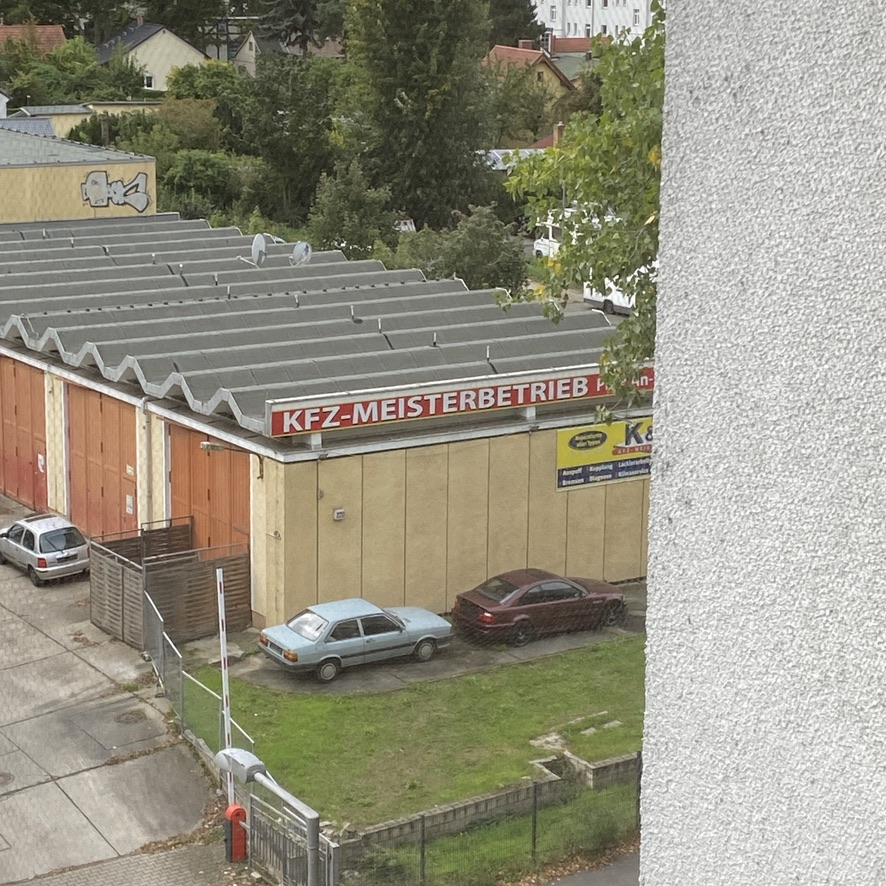
\includegraphics[width=\linewidth]{img/sample2.jpeg}
	  \caption{A scenery}
	\end{subfigure}
	\begin{subfigure}[b]{0.4\linewidth}
		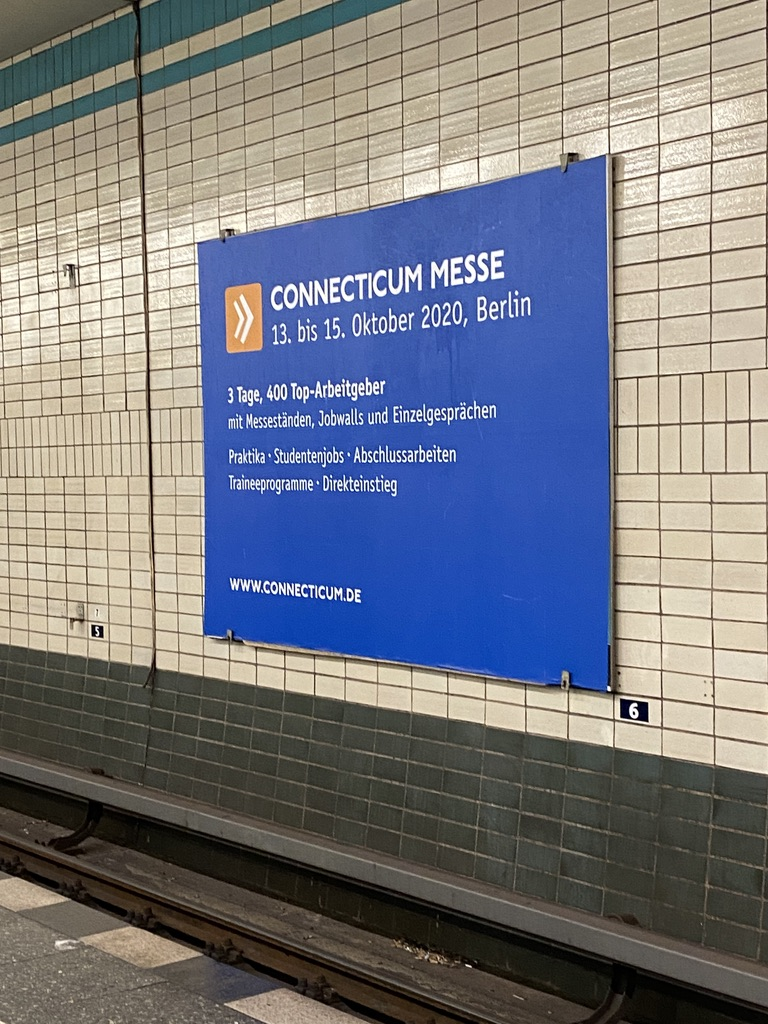
\includegraphics[width=\linewidth]{img/sample3.jpeg}
		\caption{A billboard}
	  \end{subfigure}
	\caption{Samples of natural scene images.}
	\label{fig:samples}
  \end{figure}

The random nature of the real world, combined with the diversity of available devices introduced some factors which make natural text detection a greater challenge than detecting structured text in documents. \cite{NaturalScene} mentioned some conditions that are found in natural scene which may significiantly impact text detection procedure. They are:
\begin{itemize}
	\item Raw sensor image and sensor noise
	\item Viewing angle
	\item Blur
	\item Lighting
	\item Resolution
	\item Non-paper objects
	\item Non-planar objects
\end{itemize}
Although devices have evolved to a point where most of handheld devices are capable of shooting in a high resolution, low-end handheld cameras and older models still struggle in this sector.
Uncontrolled environment, combined with the possible lack of stabilization from the equipment can cause blur \citep{Rosebrockeast}. Also, there are countless factors such as the time of the day, weather, camera flash, and many others which may impact the lighting conditions, further hindering the ability to detect text. Non-paper objects such as glass and plastic may reflect images, and non-planar objects such as text wrapped around a bottle becomes distorted and deformed \citep{Rosebrockeast}.
Additionally, there might be patterns that are extremely similar to text, or occlusions caused by foreign objects, which may potentially lead to confusion and mistakes \citep{LongEtAl}.
% section challenges (end)

\clearpage

\section{Methodology} % (fold)
\label{sec:methodology}
\subsection{Overview of EAST} % (fold)
\label{sub:overvieweast}
According to \cite{EastZhouEtAl}, the key component of EAST is a neural network model, which is trained to directly predict the existence of text instances and their geometries from full images \citep{EastZhouEtAl}.
Hence, the abbreviation EAST: Efficient and Accurate Scene Text Detector.
\begin{figure}[hbt!]
	\centering
	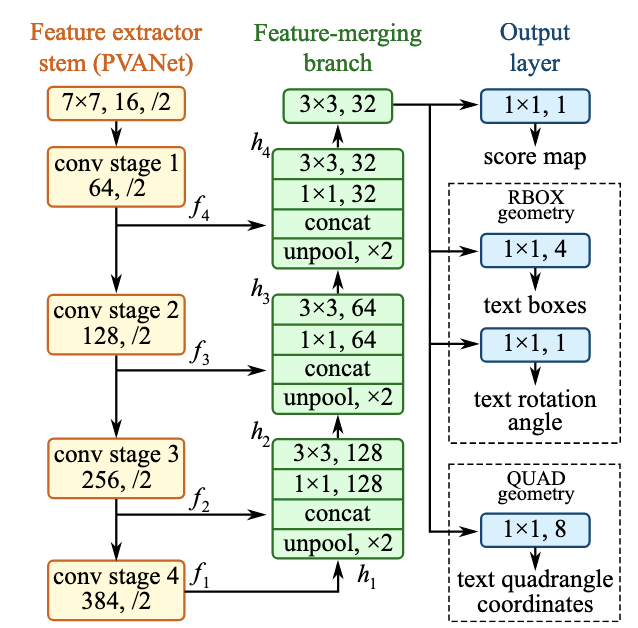
\includegraphics[width=0.5\textwidth]{img/eaststructure.png}
	\caption{Schematic view of EAST, adopted from Figure 3 of~\protect\cite{EastZhouEtAl}}
	\label{fig:east1}
\end{figure}

As claimed by \cite{EastZhouEtAl}, EAST is among the most efficient text detectors that achieve state-of-the-art performance on benchmarks.
The idea of the network is adopted from U-shape (or U-net) \citep{unet}, which simultaneously merges the feature maps and keeps the upsampling branches small. 

The end result is a network which is able to utilize different levels of features while keeping the computation cost low \citep{EastZhouEtAl}.
It is capable of predicting text on 720p images, running at an average of 13 FPS. The fastest setting, which reached a speed of 16.8 FPS was achieved on a combination of their algorithm with PVANET on 720p images using NVIDIA Titan X graphics card. \citep{EastZhouEtAl}.

The network undergoes and end-to-end training using ADAM \citep{adam} optimizer. 512x512 crops from images are uniformly sampled to form a minibatch of size 24 to accelerate the learning process.
Learning rate of ADAM starts from 1e-3, decays to one-tenth every 27300 minibatches, and stops at 1e-5. The network is trained until performance stops improving \citep{EastZhouEtAl}.
% subsection overvieweast (end)

\clearpage

\subsection{Testing} % (fold)
\label{sub:testing}
The test will be done on three different data groups with varying degrees of difficulties. They will be divided into easy, intermediate, and hard. The aim of this test is to see how the method performs on detecting text in natural scene images, determined by the detection rate and speed. It will be ran on a single NVIDIA RTX 2060 Super.

The grouping criteria of the dataset are as follow: the 'easy' group consists of images which are not natural scene. These are scanned images from item packaging and books.
\begin{figure}[hbt!]
	\centering
	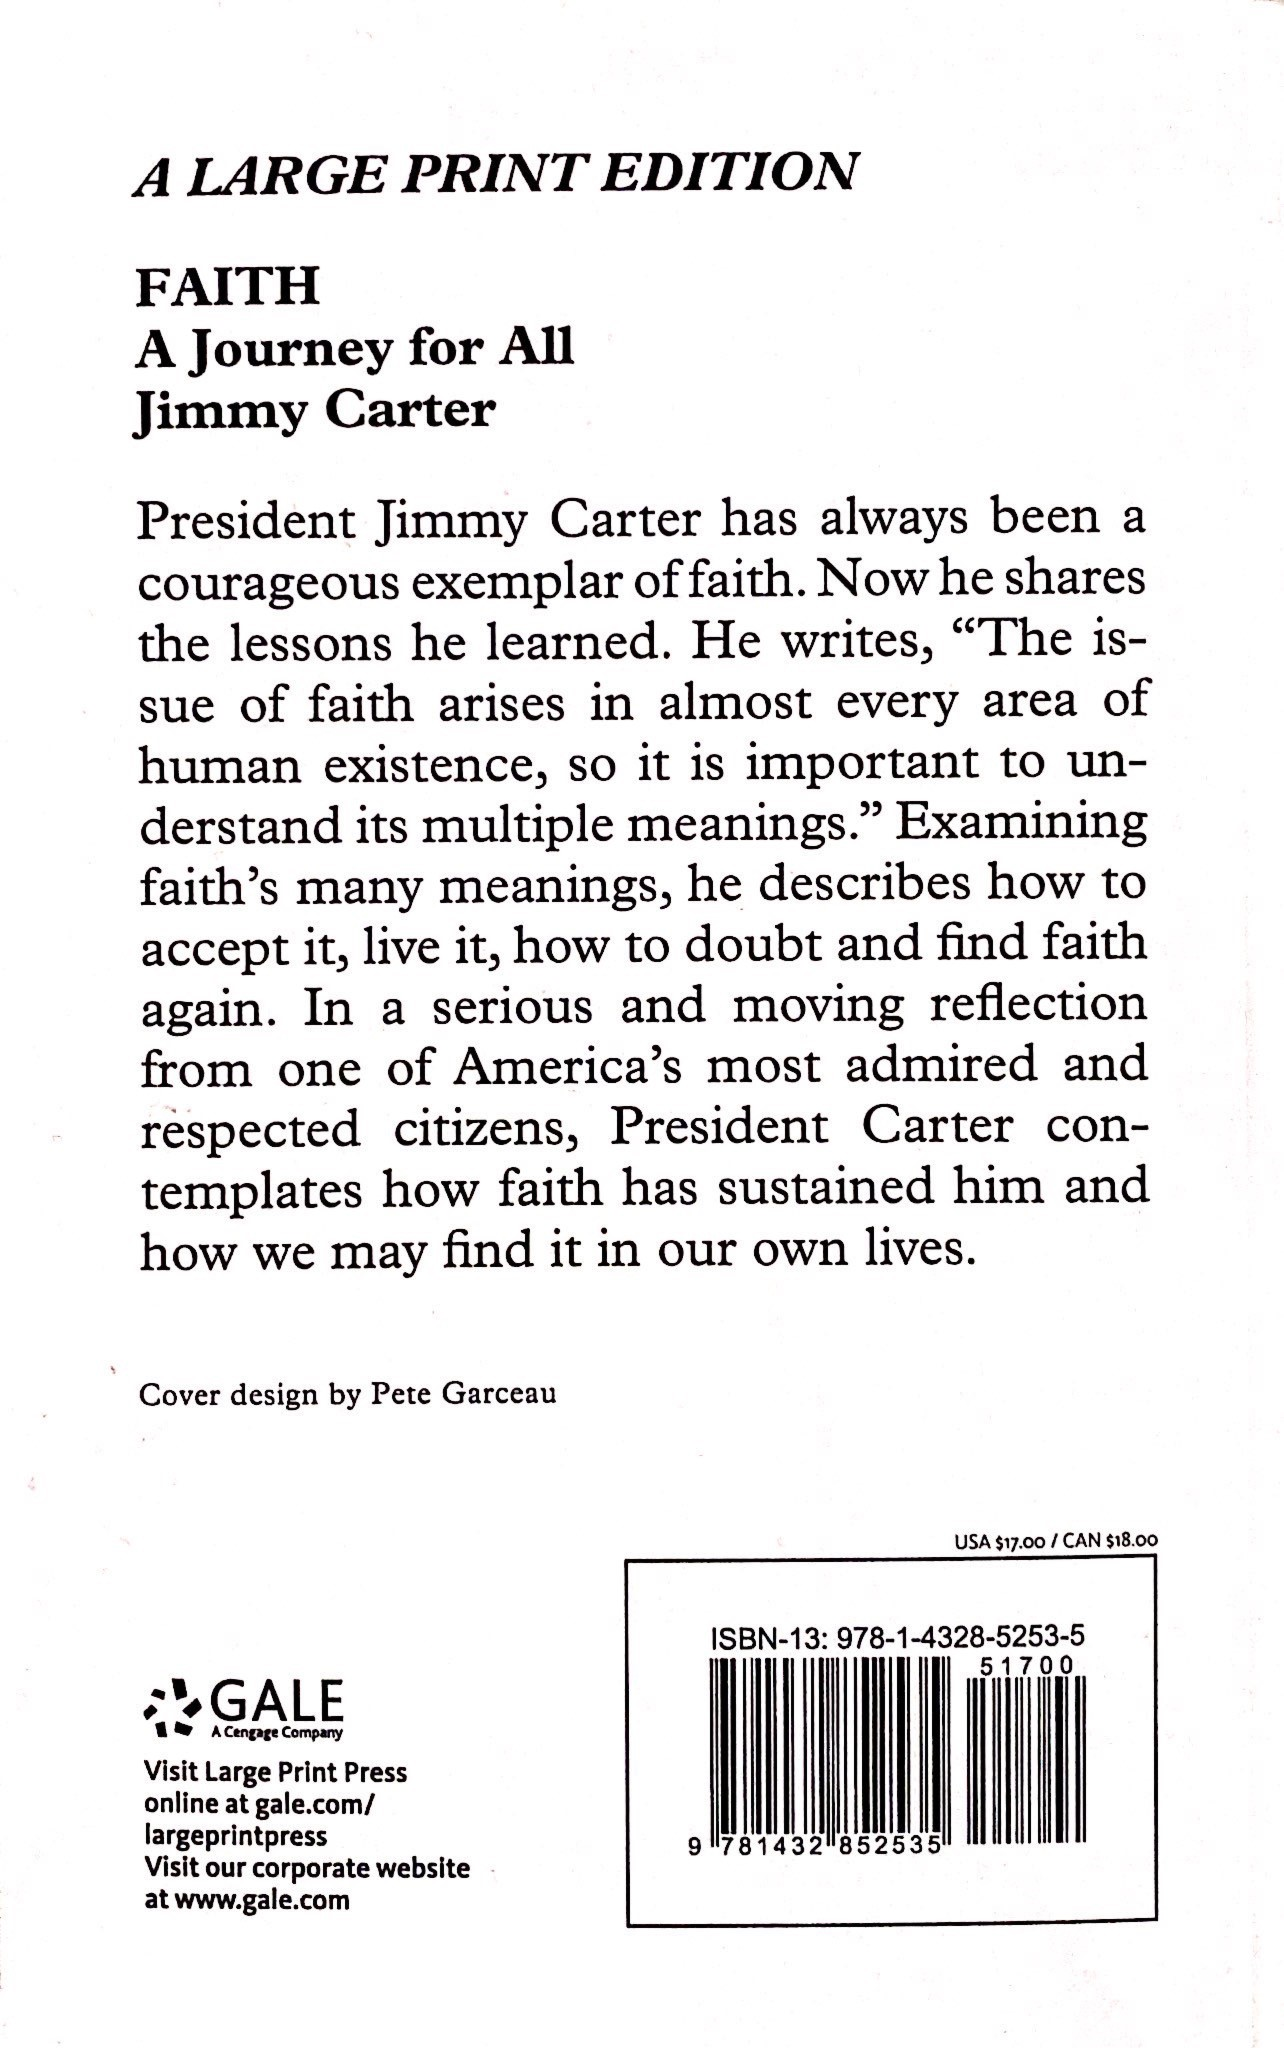
\includegraphics[width=0.5\textwidth]{img/sampleeasy.JPG}
	\caption{A sample image from the 'easy' group}
	\label{fig:sampleeasy}
\end{figure}

The 'intermediate' group is classified as such because it contains natural scene images which are taken relatively close to the camera with optimal lighting conditions and one obstructing factor from the following:
\begin{itemize}
	\item Condensed, small texts
	\item Mirroring effects
	\item Movement
	\item Object is far from the camera
	\item Old camera effect
	\item Poor lighting conditions
	\item Text is obstructed behind something else
	\item Wrapped text / distorted text
\end{itemize}

The 'hard' group consists of natural scene images with two or more of the aforementioned factors.
\begin{figure}[h!]
	\centering
	\begin{subfigure}[b]{0.4\linewidth}
		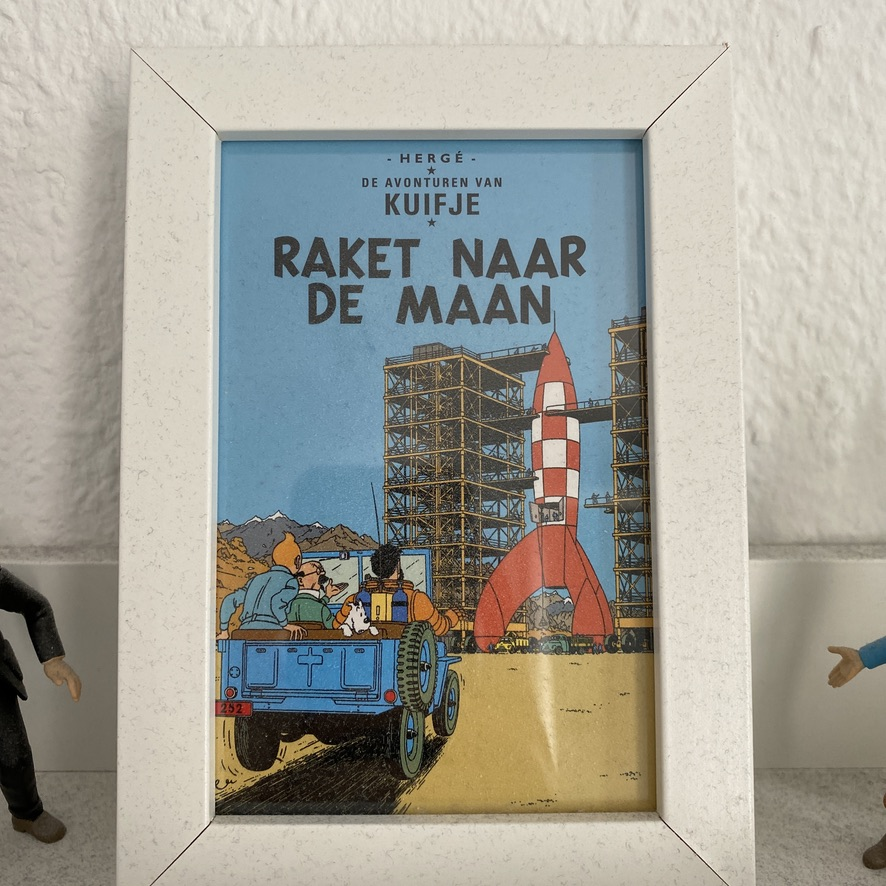
\includegraphics[width=\linewidth]{img/sample1.jpeg}
		\caption{A sample image from the 'intermediate' group}
	\end{subfigure}
	\begin{subfigure}[b]{0.4\linewidth}
		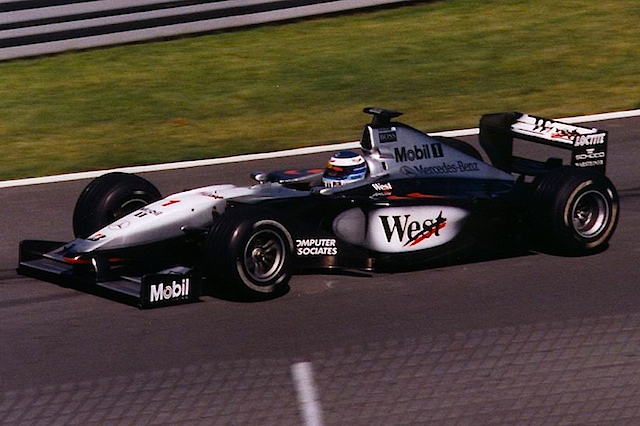
\includegraphics[width=\linewidth]{img/samplehard.JPG}
		\caption{A sample image from the 'hard' group, from \cite{mikapic}}
	\end{subfigure}
	\caption{Samples of image from intermediate and hard dataset group.}
	\label{fig:samples_dataset}
  \end{figure}

Each dataset group contains approximately six images with similar criteria, which are grouped in their own folders. The images will be resized to a multiple of 32. For the sake of consistency, every image will be resized to a square of 640 pixels regardless of their original dimensions.

A binary large object will be created for every image and passed into the network. A forward pass will then be executed, which returns two maps: scores and geometry. 
Scores will be the probability of a text being present in a region and geometry will be used to derive the bounding box coordinates of text in the input images \citep{Rosebrockeast}.

For each rows in the scores map, the probabilities and geometrical data containing potential bounding box coordinates will be extracted.
For each column in the scores map, the algorithm will predict whether the score has a sufficient probability to contain a text. It will do some calculations and get the width and length of the bounding box from the geometry volume. Both the start and end coordinates will be calculated and they will be added into a list along with the probability score.

Non-maxima suppresion will be used to overwrite weak bounding boxes. The remaining boxes will be scaled using the image ratio and drawn onto the original image.

The network will then run through each dataset group and the total time that it needs to detect everything will be counted and save.
The resulting images and total time will be presented in the following section.

% subsection testing (end)
% section methodology (end)
\clearpage
\section{Results and Evaluation} % (fold)
\label{sec:evaluation}
As the name suggests, EAST is an efficient and accurate scene text detector \citep{EastZhouEtAl}. The aim of this section is to present the results obtained from the previous section and evaluate them based on the time needed and its detection rate. The presented results will be of the best and the worst from each dataset group.
\subsection{'Easy' Group} % (fold)
\label{sub:easy}
The easy group was done in approximately 2.8307597637176514 seconds. The following are the best and worst detected image respectively:
\begin{figure}[h!]
	\centering
	\begin{subfigure}[b]{0.4\linewidth}
		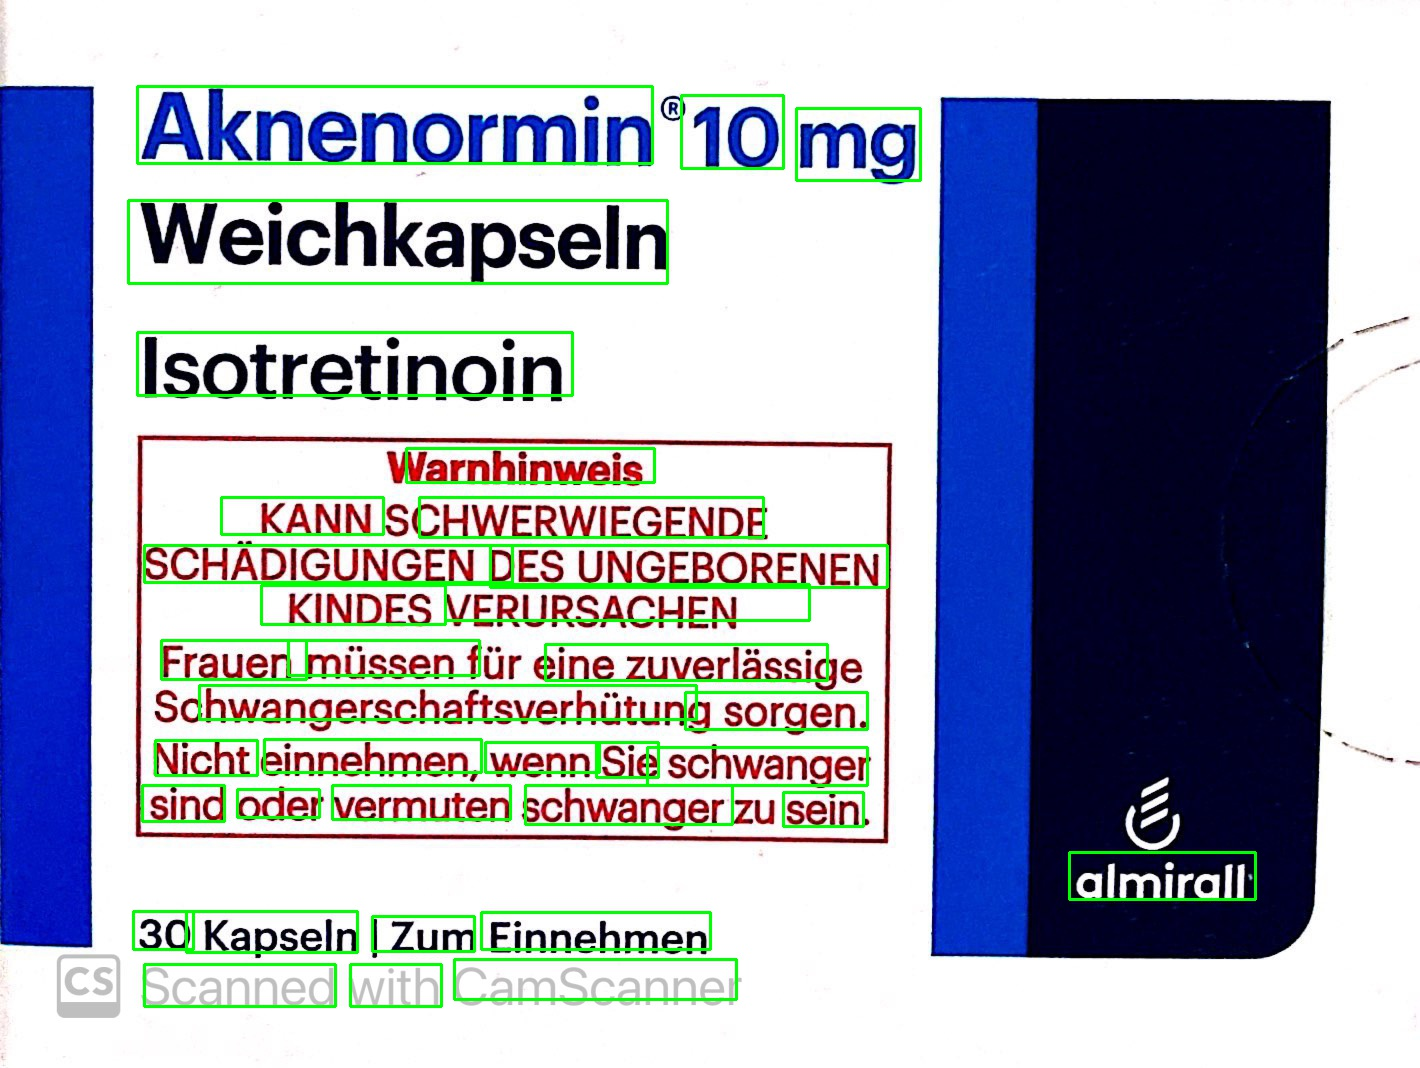
\includegraphics[width=\linewidth]{jupyter/results/easy/sample_output_3.jpeg}
		\caption{The best-detected image.}
	\end{subfigure}
	\begin{subfigure}[b]{0.4\linewidth}
		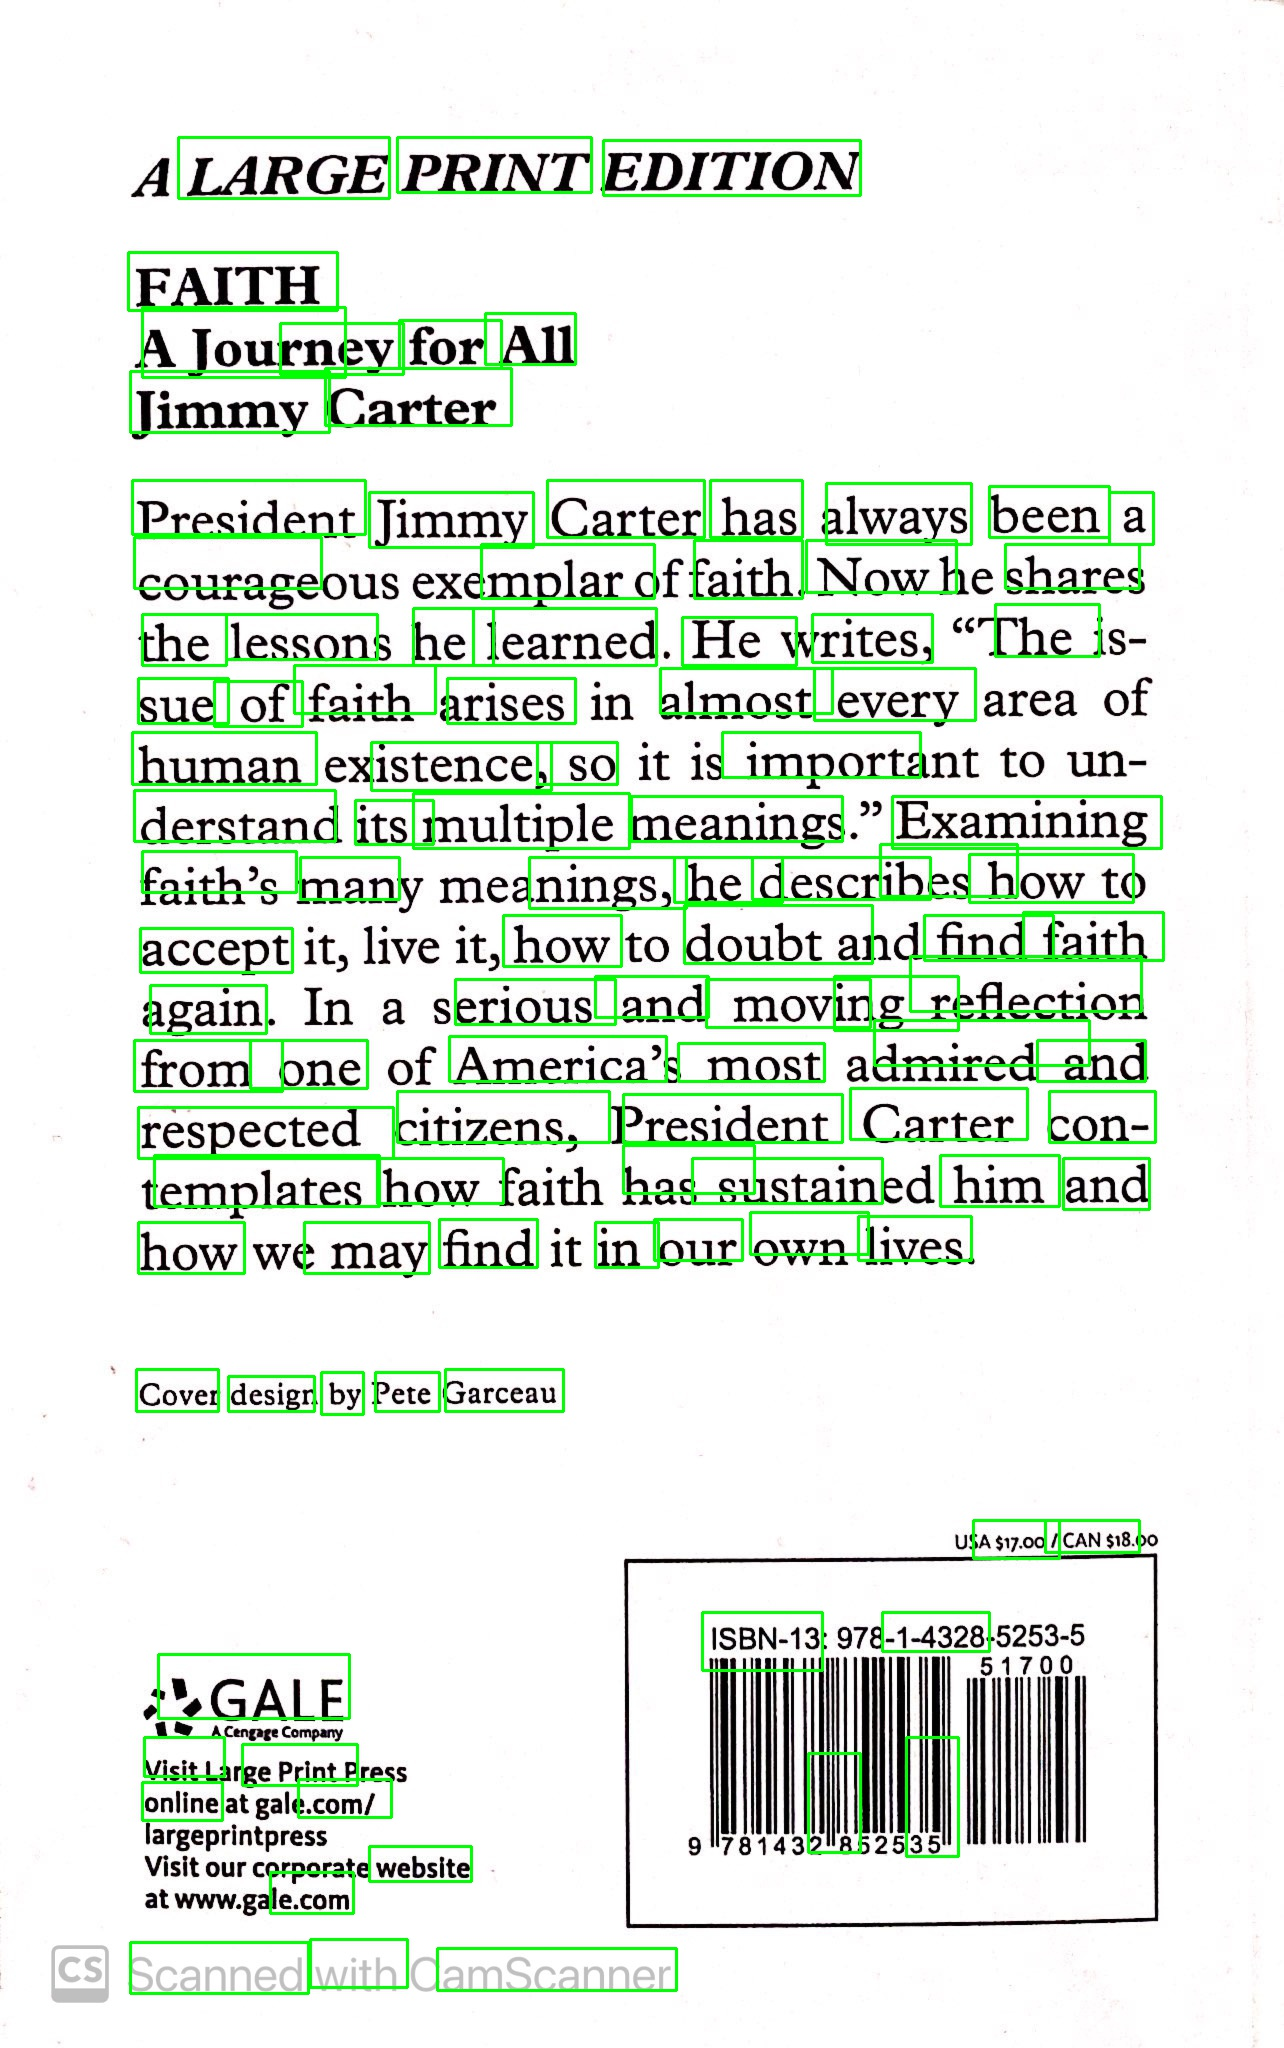
\includegraphics[width=\linewidth]{jupyter/results/easy/sample_output_0.jpeg}
		\caption{The worst-detected image.}
	\end{subfigure}
	\caption{Best and worst detected images from the easy dataset group.}
	\label{fig:sampleeasybestworst}
  \end{figure}


As seen above, every single text in the best image is detected, including the faint watermark at the very bottom. Considering that this is a scanned image, it is no surprise that this was a walk in a park for the algorithm. The characters are written clearly and there are no presence of any hindrance whatsoever. The only hiccup in this image is the umlaut in the 'für' which was unable to be detected.

In the worst-detected image, the algorithm skipped many words. After a deeper look, it can be noticed that the words skipped are short words such as 'in', 'it', etc. The hypothesis for this is that the bounding box for these words overlap with the neighboring box, which is stronger. The cramped nature of the image does not help very much either. Therefore, the box is probably eliminated in the non-maxima suppresion stage.
% subsection easy (end)
\subsection{'Intermediate' Group} % (fold)
\label{sub:inter}
The intermediate group was done in approximately 2.682370662689209 seconds. The following are the best and worst detected image respectively:
\begin{figure}[h!]
	\centering
	\begin{subfigure}[b]{0.4\linewidth}
		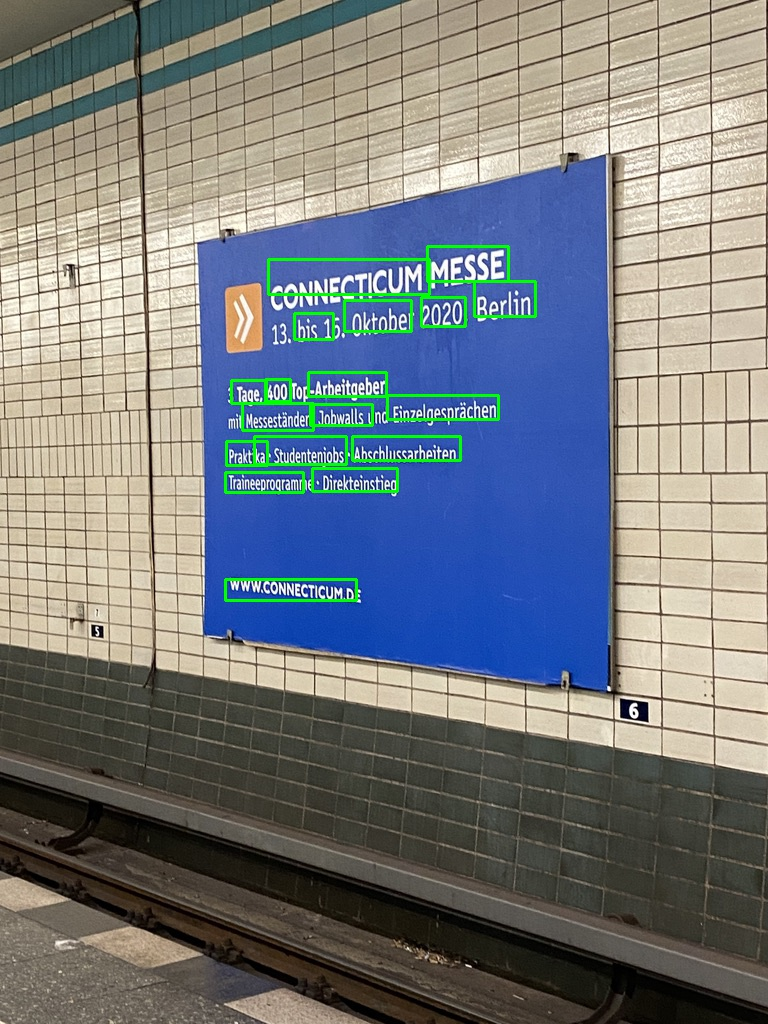
\includegraphics[width=\linewidth]{jupyter/results/inter/sample_output_3.jpeg}
		\caption{The best-detected image.}
	\end{subfigure}
	\begin{subfigure}[b]{0.4\linewidth}
		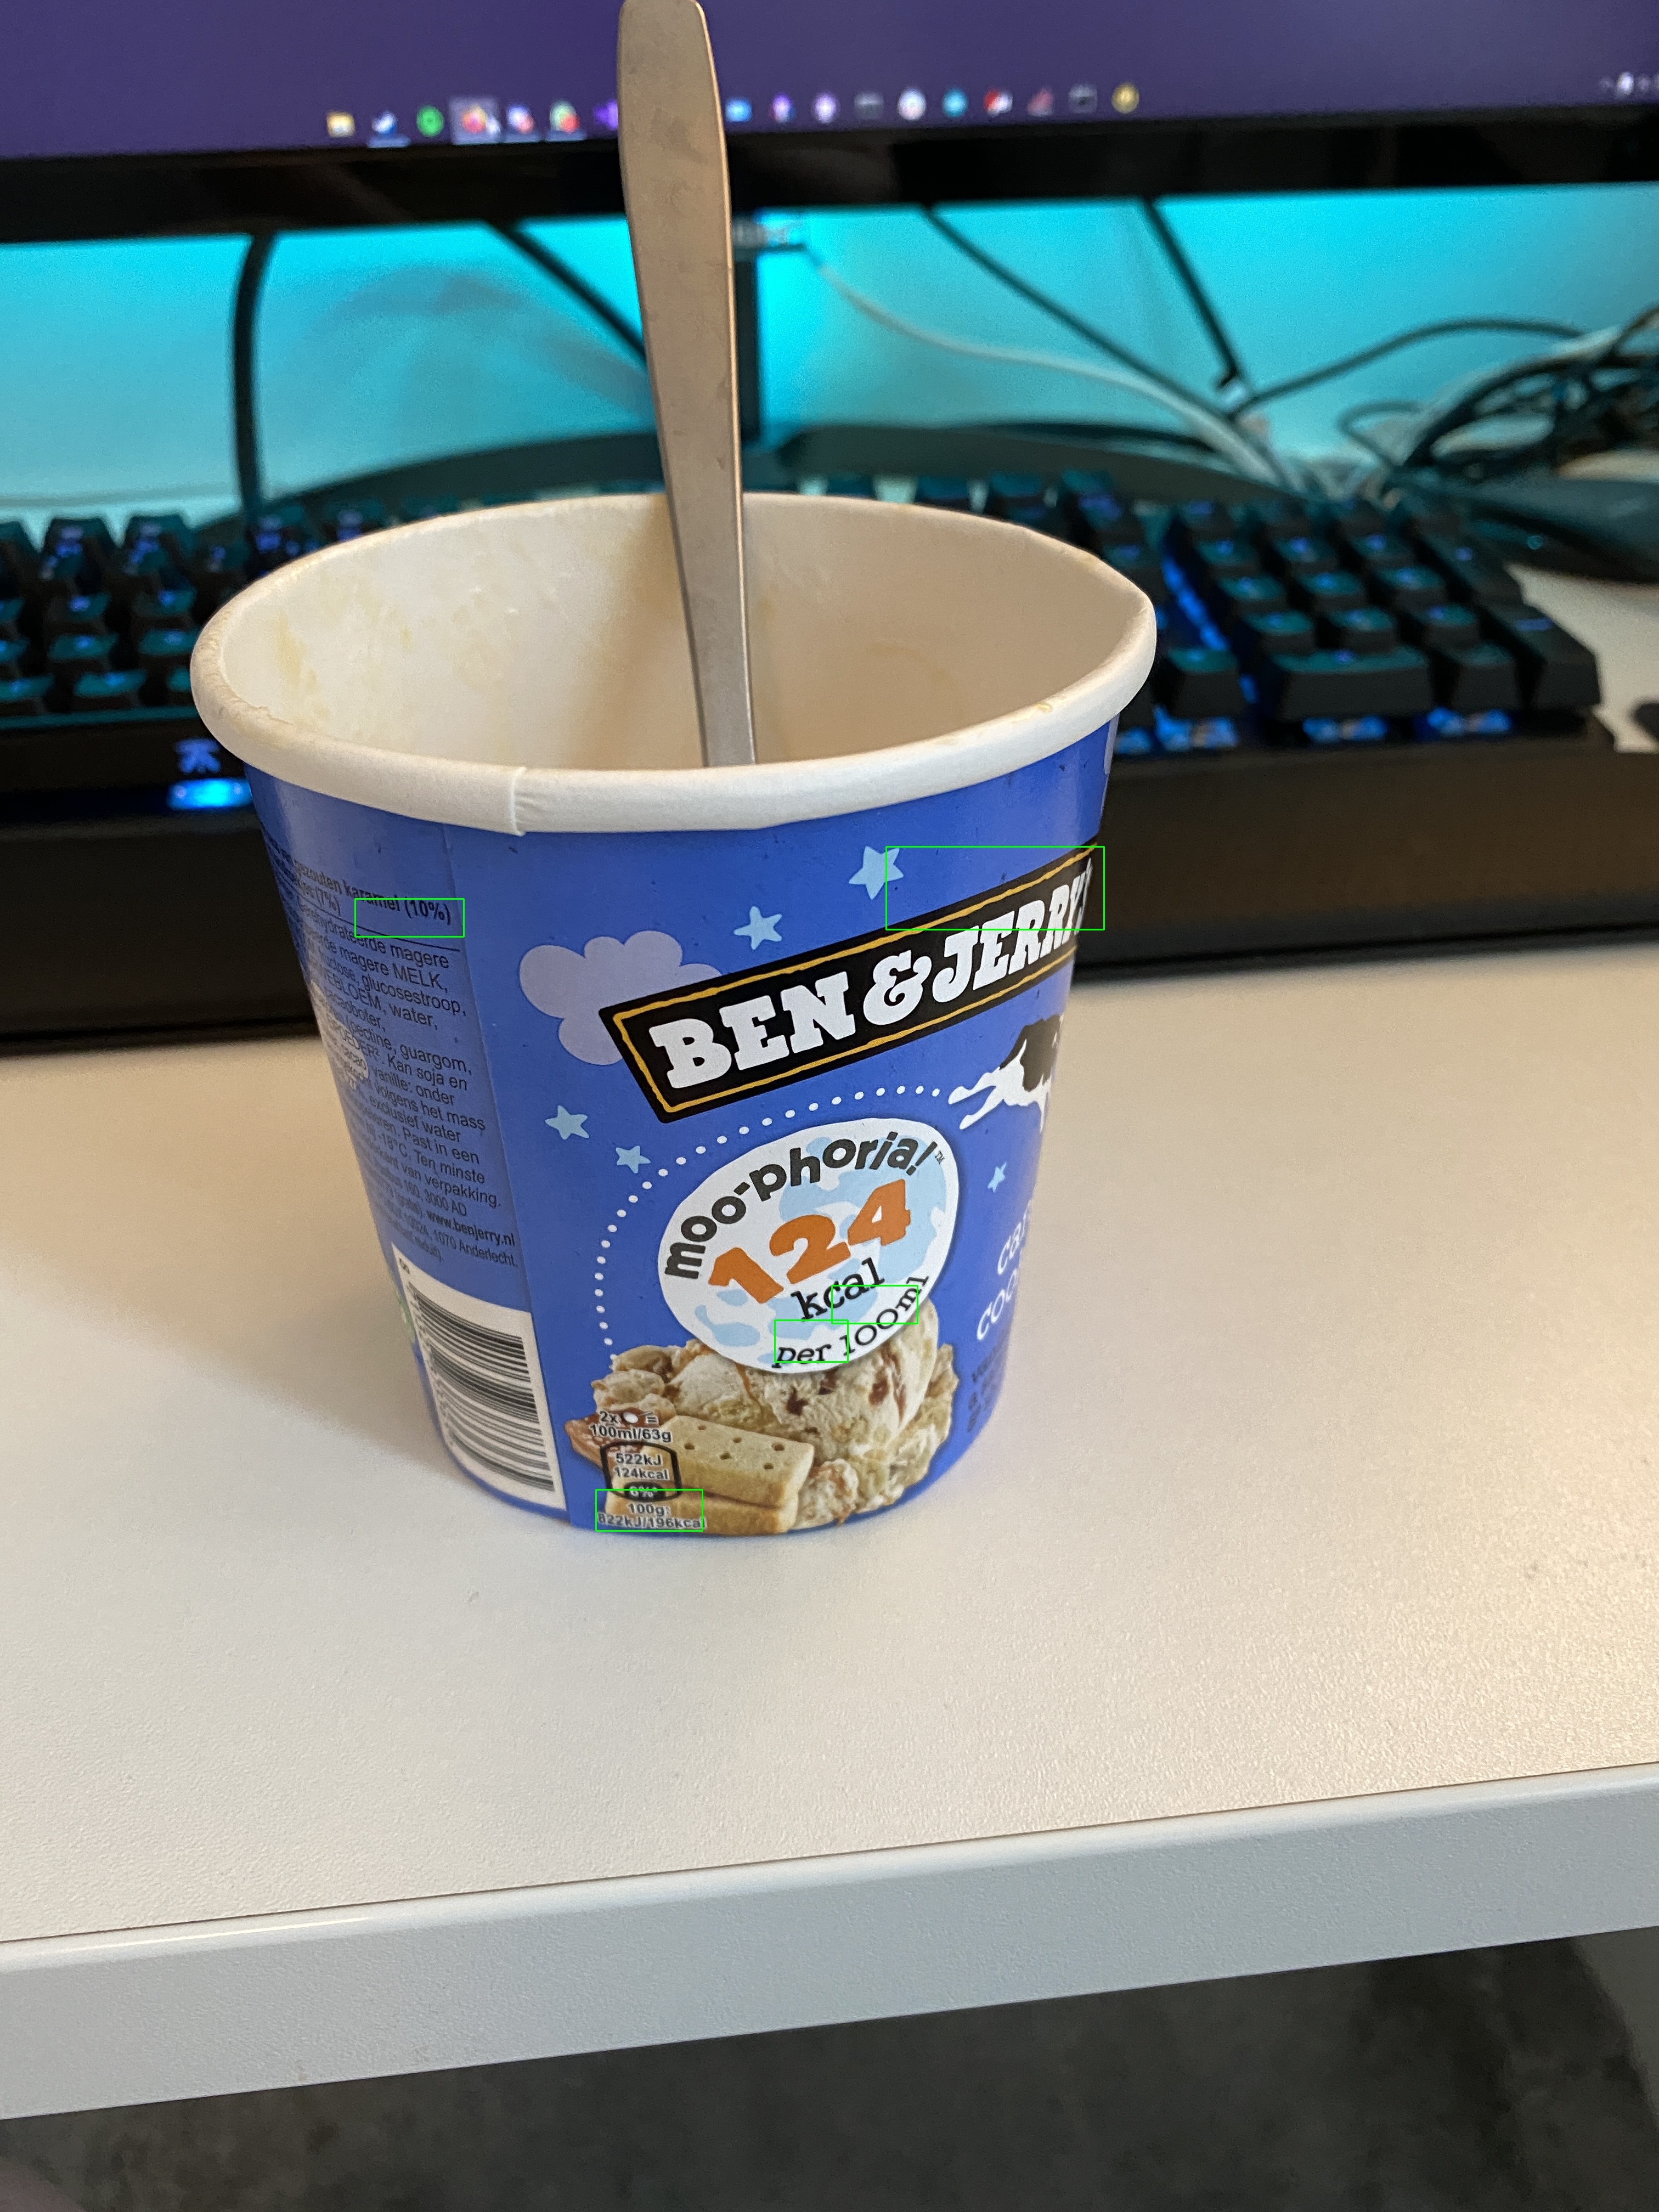
\includegraphics[width=\linewidth]{jupyter/results/inter/sample_output_2.jpeg}
		\caption{The worst-detected image.}
	\end{subfigure}
	\caption{Best and worst detected images from the intermediate dataset group.}
	\label{fig:sampleinterbestworst}
  \end{figure}

In this group, the random nature of the world is introduced. However, the images are still under optimal lighting conditions and the texts are perfectly readable to the human eye.
In the best-detected image, almost every text is detected except for two short words. Reason for this might be the same as stated in section \ref{sub:inter}, with the addition of distance. The worst-detected image is disappointing. The algorithm only managed to detect 5 points, the most noticeable being 'JERRY' and the calorie counter. The appalling results can be attributed to the way the texts wrap and distort themselves around the tub. Combined with the non-standard font that this particular brand is using, this may throw the algorithm off.
% subsection inter (end)
\clearpage

\subsection{'Hard' Group} % (fold)
\label{sub:hard}
The hard group was done in approximately 2.573026180267334 seconds. The following are the best and worst detected image respectively:
\begin{figure}[h!]
	\centering
	\begin{subfigure}[b]{0.4\linewidth}
		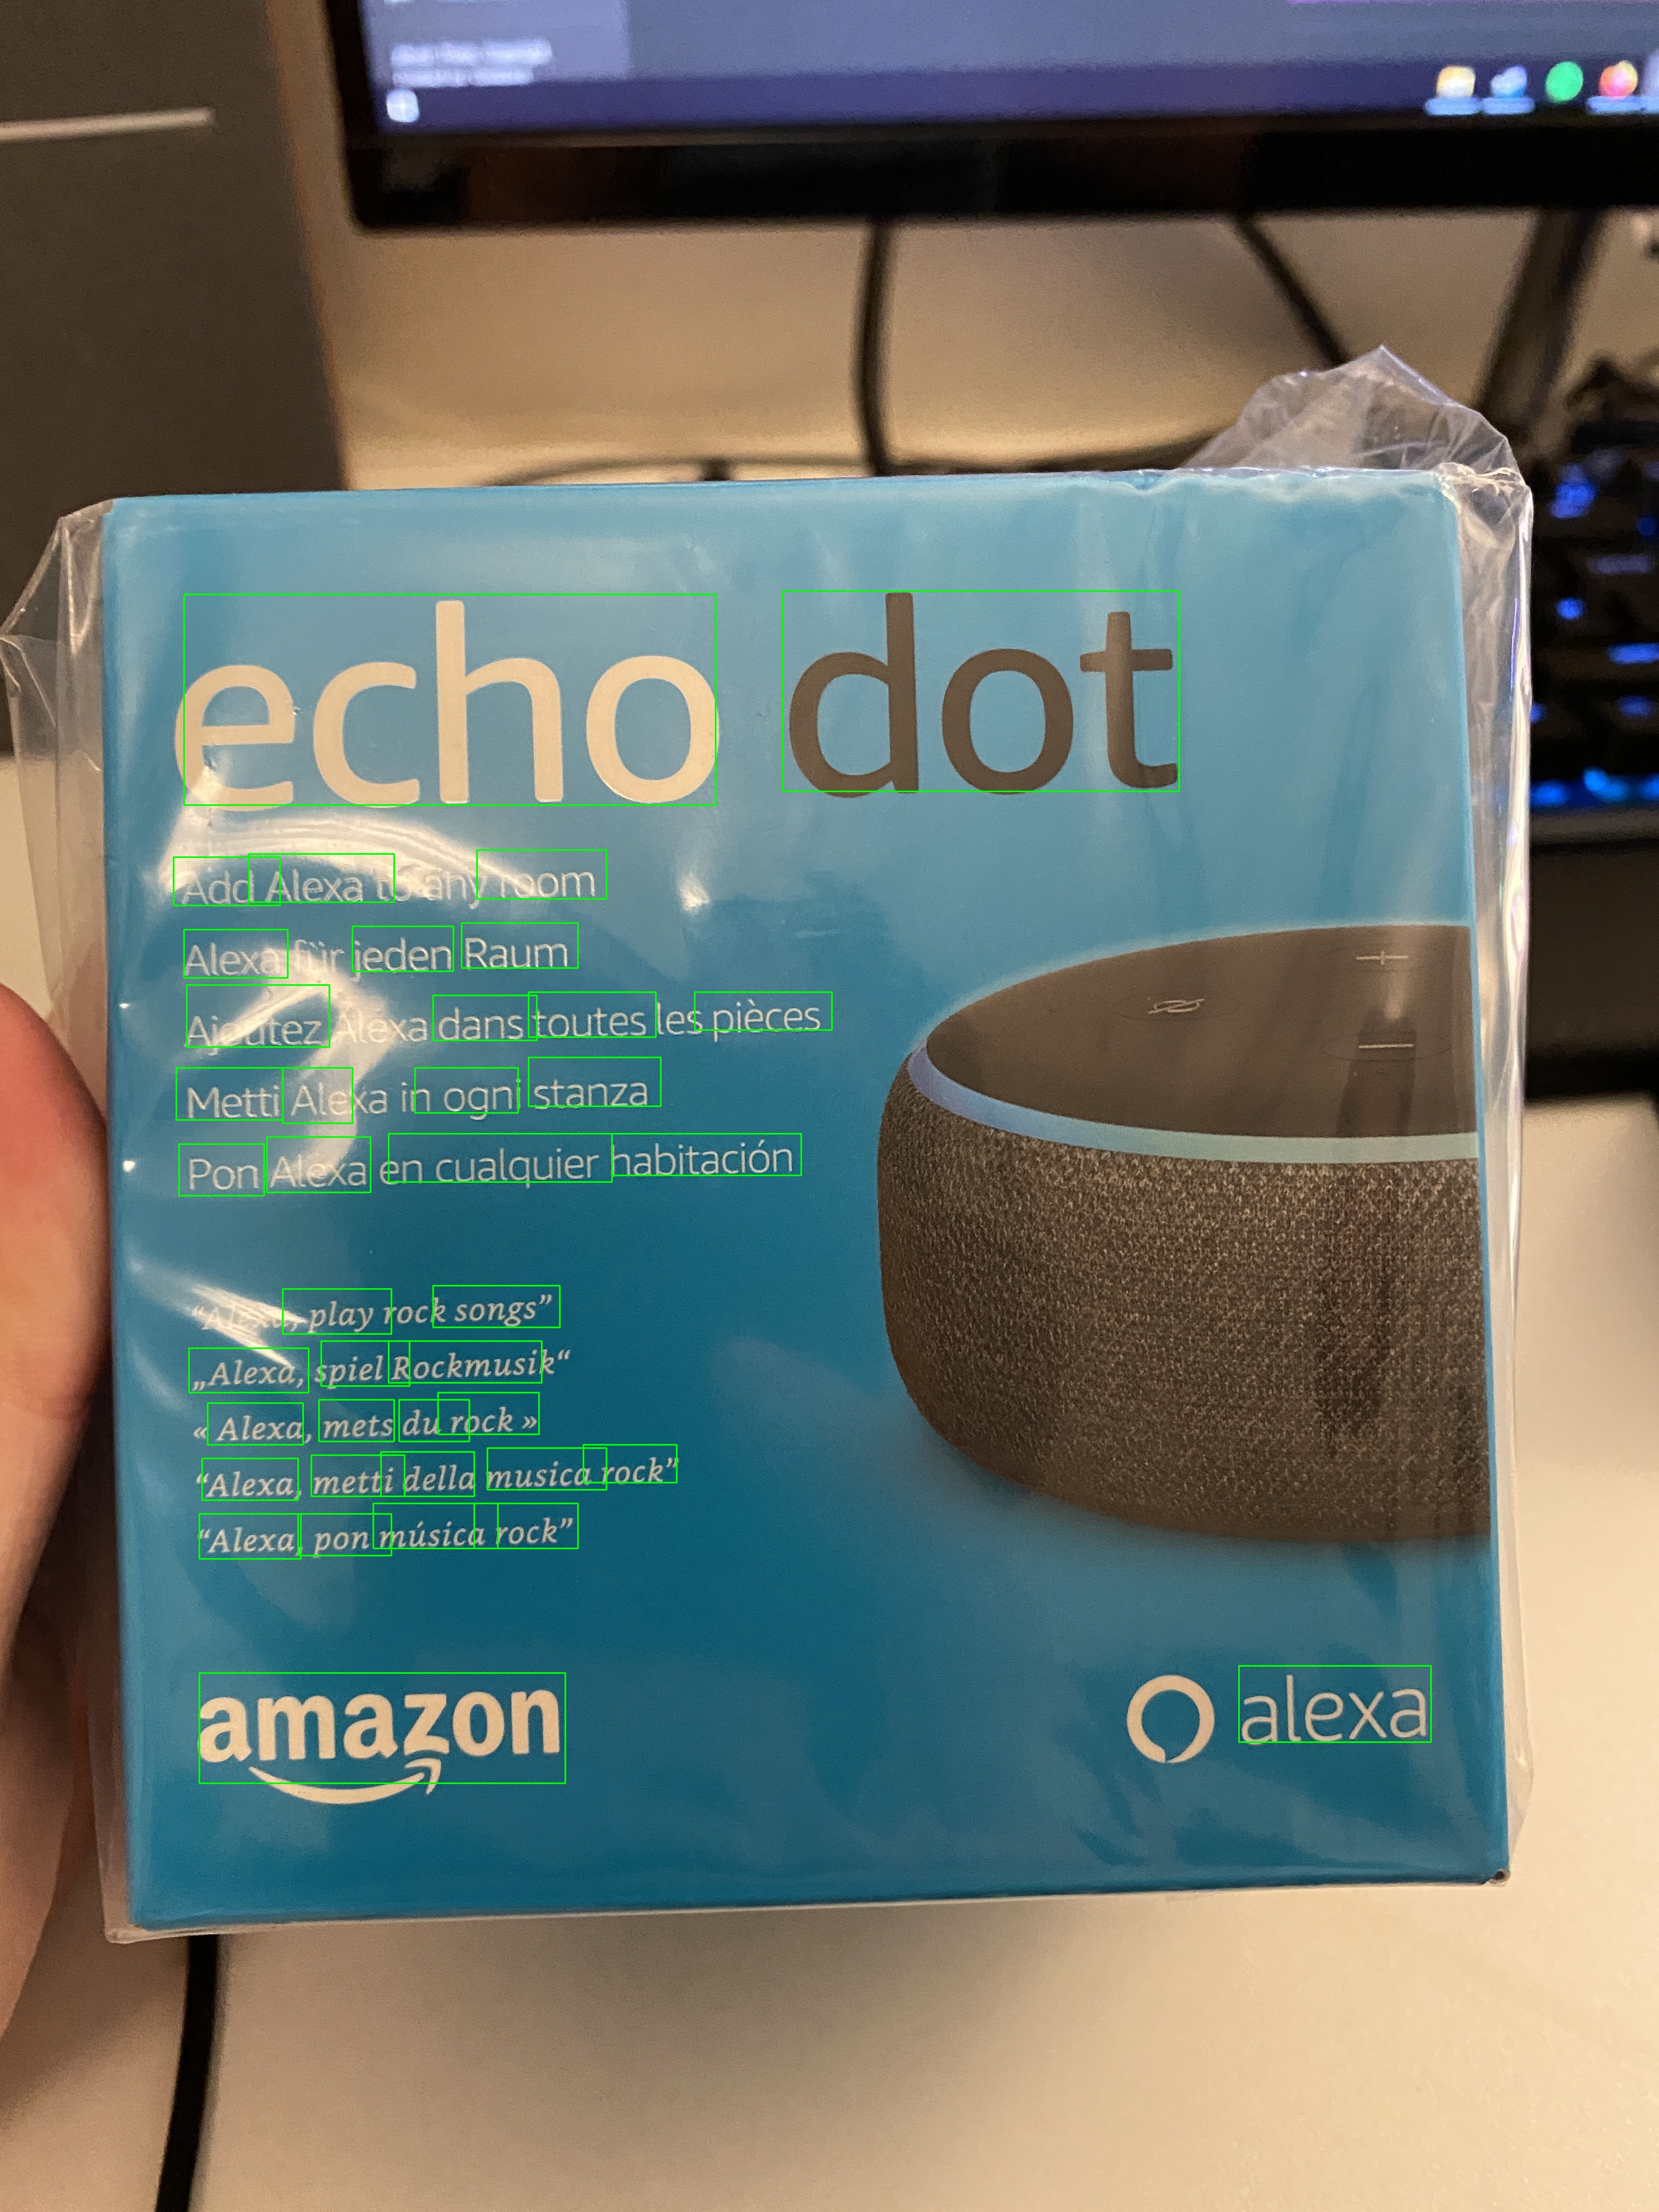
\includegraphics[width=\linewidth]{jupyter/results/hard/sample_output_1.jpeg}
		\caption{The best-detected image.}
	\end{subfigure}
	\begin{subfigure}[b]{0.4\linewidth}
		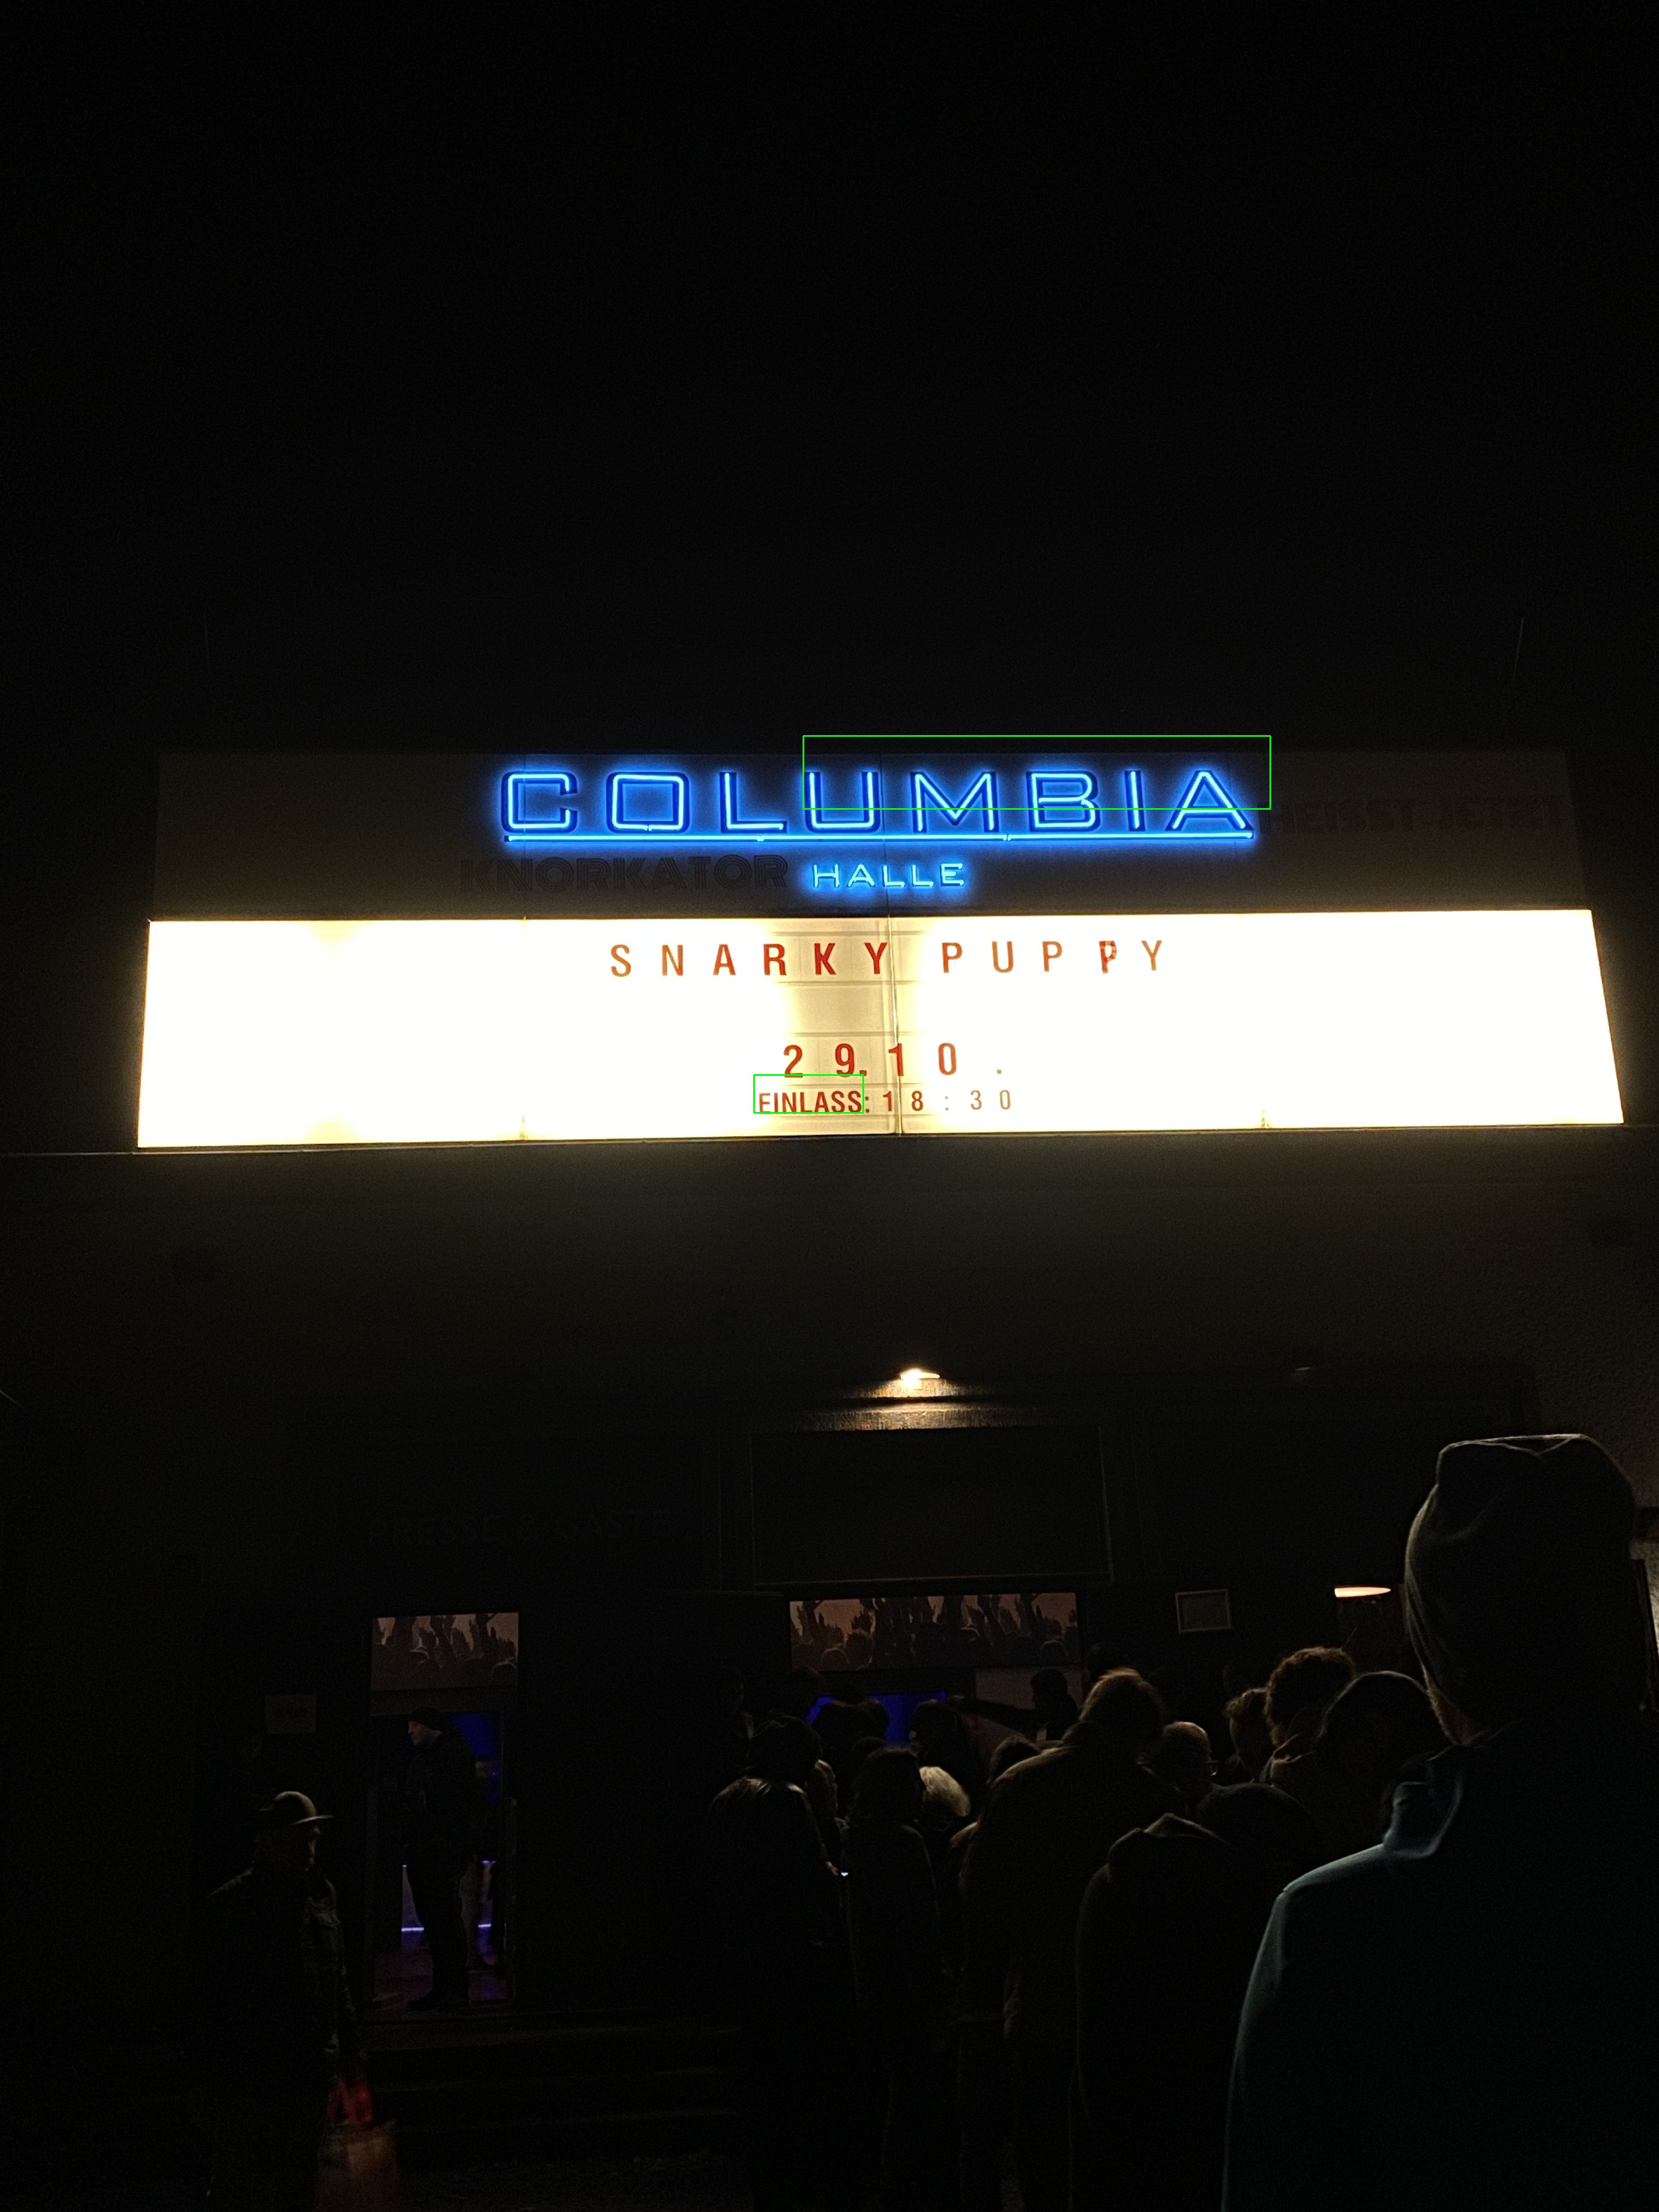
\includegraphics[width=\linewidth]{jupyter/results/hard/sample_output_0.jpeg}
		\caption{The worst-detected image.}
	\end{subfigure}
	\caption{Best and worst detected images from the hard dataset group.}
	\label{fig:samplehardbestworst}
  \end{figure}

In this group, the algorithm is tested further than before. Every image in this group has at least two or more hindering factors mentioned in section \ref{sub:testing}. 

As seen above in the first image, the text is obstructed underneath a layer of plastic covering and it also has reflections of a light and a shadow. Surprisingly, the algorithm managed to detect almost every text in this image despite all the hindrance. Exception are the words which are directly under the reflection, but that is excused as it is practically unrecognizable.

The second image was taken in the dark of night, with the neon sign emitting its own light, creating a glowing effect which may throw the algorithm off. As a result, only two boxes were present. The word 'SNARKY PUPPY' was positioned above an extremely bright white light, which were in stark contrast with the pitch-black background of the night sky.

The harder the image, the faster the time taken to detect the words. This group was the fastest to detect. It may sound ironic, but it was because there were less detection points due to the difficulty of the image. As the algorithm skipped the region, it did not need to do anything there and went straight to the next probability-region, therefore it is faster.
% subsection hard (end)
% section evaluation (end)
\clearpage
\section{Conclusion} % (fold)
\label{sec:conclusion}
The EAST scene text detector was chosen for it's speed, efficiency, and accuracy. It has been proven that it was fast enough in that it went through the three groups of six images, to a total of 18, on an average time of 0.44 seconds per image. 

Scanned images were a walk in the park for the detector. It detected almost every text found in the image with only minor mistakes and within a rapid timeframe.

On natural scene images, the algorithm struggles more than on scanned images. These are due to the fact that there are many factors which may interfere with the detection process in natural scene images, such as lighting, blur, reflection, etc. However, given the right image, EAST can be very efficient and accurate in that it detects every text in the image within an exceptionally fast time.
% section conclusion (end)
\clearpage
\newpage 

\bibliographystyle{natdin}
	\bibliography{references} % expects file "references.bib"
	\addcontentsline{toc}{section}{References}
\end{document}